\chapter{Grammar of Graphics Tools}
The Grammar of Graphics by Leland Wilkinson is a framework that provides a unique foundation for producing almost every quantitative graphic found in scientific journals, newspapers, statistical packages, and data visualization systems.
It follows a layered approach to describe and construct visualizations or graphics, and it is a system of rules for generating valid statements in a language, making it possible for people to communicate accurately and concisely \cite{GrammarGraphics2005}.
In this section we are going to take a look at the different layers of the Grammar of Graphics and construct visualizations using the framework at hand.

\section*{The Layers: An Overview}
The Grammar of Graphics follows a layered approach to describe and construct visualizations or graphics. It provides a common language for thinking about the ways that design choices are made in visualization, describing everything from the data used to the visual channels displayed on the marks, and how data is converted into those channels.
\begin{figure}[h]
    \centering
    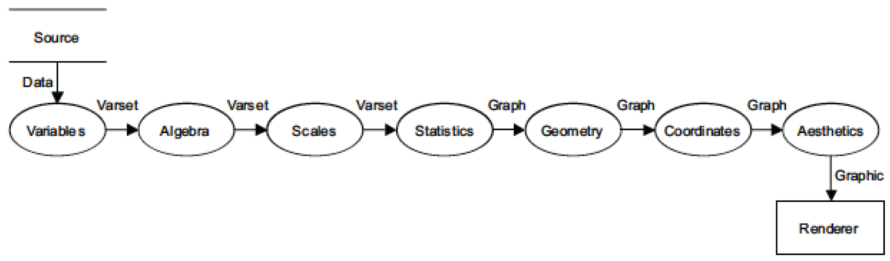
\includegraphics[width=\textwidth]{figures/grammar_flow.png}
    \caption{Grammar of Graphics Flow \cite{wilkinsonHowMakePie2005}}
\end{figure}

In the graphic above the layered approach is displayed. After the data was loaded, different transformations 
get applied to stick together the features that should be displayed. Each step yields a new ``varset'' up until
the Statistics layer. This layer is responsible for calculating the statistical properties of the data. The succeeding
layers are responsible for visual modifications which at the end form a graphic.

\captionsetup{justification=centering}

\subsection*{Data}
\begin{minipage}[t]{0.6\textwidth}
    \vspace{0pt}
    In the first step, as described above, we aggregate the data we want to visualize.
    \hspace{1cm}
\end{minipage}%
\begin{minipage}[t]{0.4\textwidth}
    \vspace{0pt}
    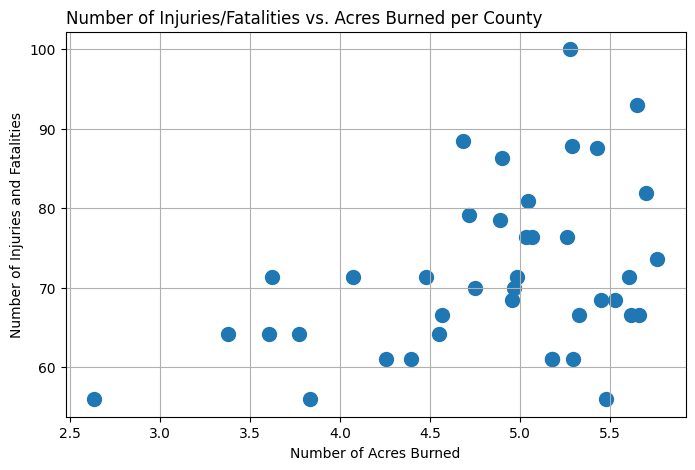
\includegraphics[width=\textwidth]{figures/gog_data.png}
    \captionof{figure}{Grammar of Graphics: Data}
\end{minipage}

\subsection*{Aesthetics}
\begin{minipage}[t]{0.6\textwidth}
    \vspace{0pt}
    In the Grammar of Graphics, the Aestehetics Layer refers to the mapping of one or more variables to one or more visual elements on the graph. This includes mapping variables to the x-axis, y-axis, and using color to differentiate different attributes. Aesthetics are essential in creating meaningful and effective visualizations \cite{wilkinsonAesthetics2005}.
    In this example we map the \texttt{AcresBurned} variable to the x-axis and the sum of \texttt{Injuries} and \texttt{Fatalities} variables to the y-axis.
    \hspace{1cm}
\end{minipage}%
\begin{minipage}[t]{0.4\textwidth}
    \vspace{0pt}
    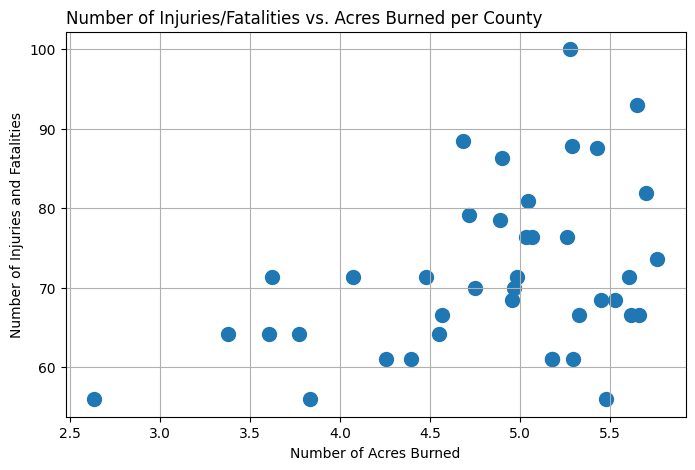
\includegraphics[width=\textwidth]{figures/gog_data.png}
    \captionof{figure}{Grammar of Graphics: Aesthetics}
\end{minipage}

\subsection*{Scale}

\subsection*{Geometry}

\subsection*{Statistics}

\subsection*{Facets}

\subsection*{Coordinates}